\chapter{\IfLanguageName{dutch}{Fase 1 - Directe implementatie}{Fase 1 - Direct Implementation}}
\label{ch:fase1}

In dit hoofdstuk doorlopen we hoe in een bestaand ERP-systeem een nieuw bedrijfsproces geïmplementeerd kan worden.

\section{Progress}

In fase 0 werd Progress kort vermeld. In dit hoofdstuk nemen we een diepere kijk naar wat Progress nu precies is en wat het zo een krachtig platform maakt voor businessoplossingen.

\subsection{Wie is Progress}

Progress is een Amerikaans bedrijf dat al voor 40 jaar een fundamentele rol speelt in de wereld van bedrijfssoftware. Hun missie is simpelweg: De ontwikkeling van bedrijfsapplicaties versnellen. 
\\
\\
Ze doen dit door hun toolbox, genaamd OpenEdge, te ontwikkelen. OpenEdge is de omvattende naam van alles dat je nodig kunt hebben om een bedrijfsapplicatie te bouwen. Database, Frameworks, Cloud servers, etc. Alles zit erin. Doordat al deze tools door dezelfde provider (Progress), worden aangeboden, heb je geen enkele last van compatibiliteitsproblemen. Dit zorgt ook voor een lagere Time-To-Value (ToV), wat in de eerste plaats ook hun missie is.
\pagebreak
\subsection{De Technologie}

\subsubsection{Advanced Bussiness language}
Openedge gebruikt hun eigen Advanced Bussiness Language (ABL). Deze high-level programmeertaal is Data-centric en staat heel dicht bij bestaande data. De structuur van de data en hoe het allemaal aan elkaar zit, is meteen gekend voor de taal. Er is geen nood aan een domeinlaag/Entity Framework om bij te houden welk object welke data heeft. het gevolg hiervan is dat transacties tussen de applicatie en database snel en efficiënt gebeuren en ook zeer diep beveiligd tegen fouten.
\\
\\
ABL is een high-level programming language. Dit betekent dat achter elke lijn die geschreven wordt, er een hele bundle code achter zit. Dit zorgt er dan ook voor dat één statement in ABL, er 100 zijn in bijvoorbeeld Java. Een voorbeeld gegeven in de officiële documentatie is deze: `A single ABL statement can bring data all the way from the application database to the user interface, or return a user's changes back to the database \autocite{Progress2026}.` Veel van de tools vermeld in OpenEdge zijn ook zelf geschreven in ABL.
\pagebreak
\subsubsection{Database}
OpenEdge heeft zijn eigen OpenEdge RDBMS systeem. Dit is kort voor Relationeel Database Management Systeem. De database die aan het middelpunt van de structuur staat is een door hen zelf ontwikkelde technologie die gespecialiseerd is in transacties.
RDBMS heeft een specifieke structuur die altijd gebruikt wordt.
\begin{figure}[H]
    \centering
    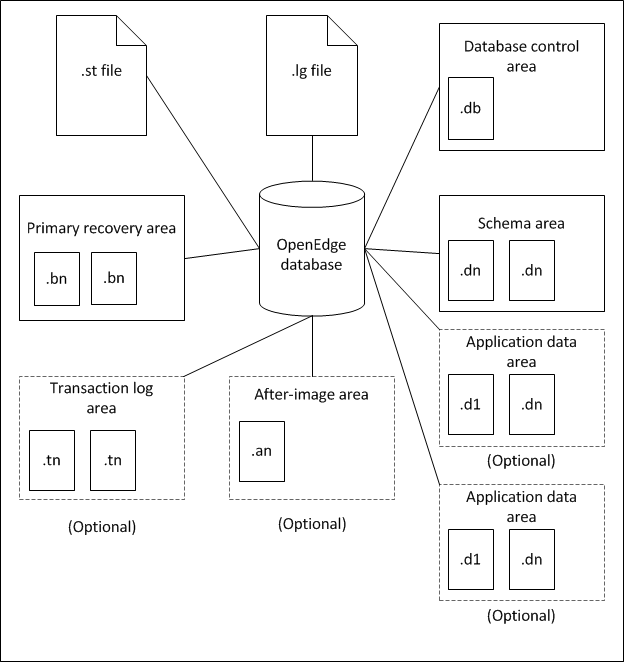
\includegraphics[width=.8\textwidth]
    {images/openedge_database}
    \caption{\label{fig:openedgedbstructuur}OpenEdge RDBMS structuur \autocite{Progress2026a}.}
\end{figure}

Ik zal niet elk deel van deze infrastructuur bespreken. \\
Het belangerijkste is de OpenEdge Database die in het midden staat. Deze database is 'record-based'. Dat betekent dat deze gefocust is op het verwerken van specifieke records (bv. een Receptiebon) en alle relaties die deze record heeft. Elke aanpassing aan een record gebeurt snel en efficiënt. 

\pagebreak

\section{Theoretische uitwerking}

TODO

\section{evaluatie}
